% ============================================================================
% Section 4: Current Work on Modelling
% Drop into the main interim report .tex between Sections 3 and 5
% ============================================================================

\section{Current Work on Modelling}

\subsection{MAPPO Architecture}

We adopt Multi-Agent Proximal Policy Optimization (MAPPO)~\cite{mappo} with
parameter sharing, following the CityLight architecture~\cite{citylight}.
Each of the 12 signalized intersections acts as an independent agent sharing a
common policy network: a 2-layer ReLU MLP with 128 hidden units mapping local
observations (queue lengths, vehicle counts, mean speeds, current phase, and
time-of-day from sumo-rl) to a softmax distribution over legal signal phases.
A centralized critic receives the concatenated observations from all agents
to estimate state value during training only. Per-feature observation
normalization is maintained via Welford running statistics. Full
hyperparameters are listed in Appendix~\ref{app:hyperparams}.

\subsection{Reward Design}

Our initial approach used a time-loss reward $r_i = -\log(1 + d_i)$, directly
targeting the proposal's primary metric. However, this sparse,
single-objective signal proved insufficient for convergence: MAPPO trained
under this reward achieved $8{,}434 \pm 589$\,s person-time-loss---\emph{worse
than even the Fixed-Time baseline} ($8{,}040 \pm 564$\,s). The policy failed
to discover useful signal coordination from delay feedback alone.

We replaced this with a multi-objective reward that combines delay reduction,
throughput encouragement, and a throughput-fairness term across intersections
(full equation in Appendix~\ref{app:reward}). Under this reward, MAPPO
improved to $7{,}101 \pm 248$\,s---a 16\% reduction over the time-loss reward
and a clear improvement over Fixed-Time, though still 25\% behind
Max-Pressure. The richer reward landscape provides gradient signal even when
delay changes are small, enabling the policy to learn meaningful coordination.

\subsection{Experimental Setup}

The study area is a Toronto OSM corridor with 12 signalized intersections and
70 TMC-calibrated car flows active over a 0--3600\,s window (see
Section~3 for data details). Episodes run for up to 300\,s at 5\,s decision
intervals; demand exhausts at approximately 285\,s. We evaluate three
controllers---MAPPO, Fixed-Time, and Max-Pressure---each over 10 random seeds.
MAPPO is trained for 30 episodes with observation normalization on an
NVIDIA RTX 4070 Laptop GPU; total compute for all reported experiments is
under 1 GPU-hour.

\subsection{Results and Analysis}

Table~\ref{tab:results} reports evaluation metrics (mean $\pm$ std across 10
seeds). Figure~\ref{fig:interim} provides a visual summary.

\begin{table}[ht]
\centering
\small
\caption{Evaluation results under the multi-objective reward (10 seeds).
  Metric definitions in Appendix~\ref{app:metrics}.}
\label{tab:results}
\begin{tabular}{@{}lcccc@{}}
\toprule
\textbf{Controller} & \textbf{Person Time} & \textbf{Avg Trip} & \textbf{Arrived} & \textbf{Delay Fairness} \\
                     & \textbf{Loss (s)}    & \textbf{Time (s)} & \textbf{Vehicles} & \textbf{(Jain)} \\
\midrule
Max-Pressure & $5{,}659 \pm 190$ & $24.1 \pm 0.6$ & $119.8 \pm 9.8$  & $0.589 \pm 0.037$ \\
MAPPO        & $7{,}101 \pm 248$ & $25.2 \pm 0.8$ & $116.9 \pm 9.8$  & $0.476 \pm 0.048$ \\
Fixed-Time   & $7{,}452 \pm 320$ & $26.4 \pm 0.8$ & $112.1 \pm 6.7$  & $0.585 \pm 0.032$ \\
\bottomrule
\end{tabular}
\end{table}

\begin{figure}[ht]
\centering
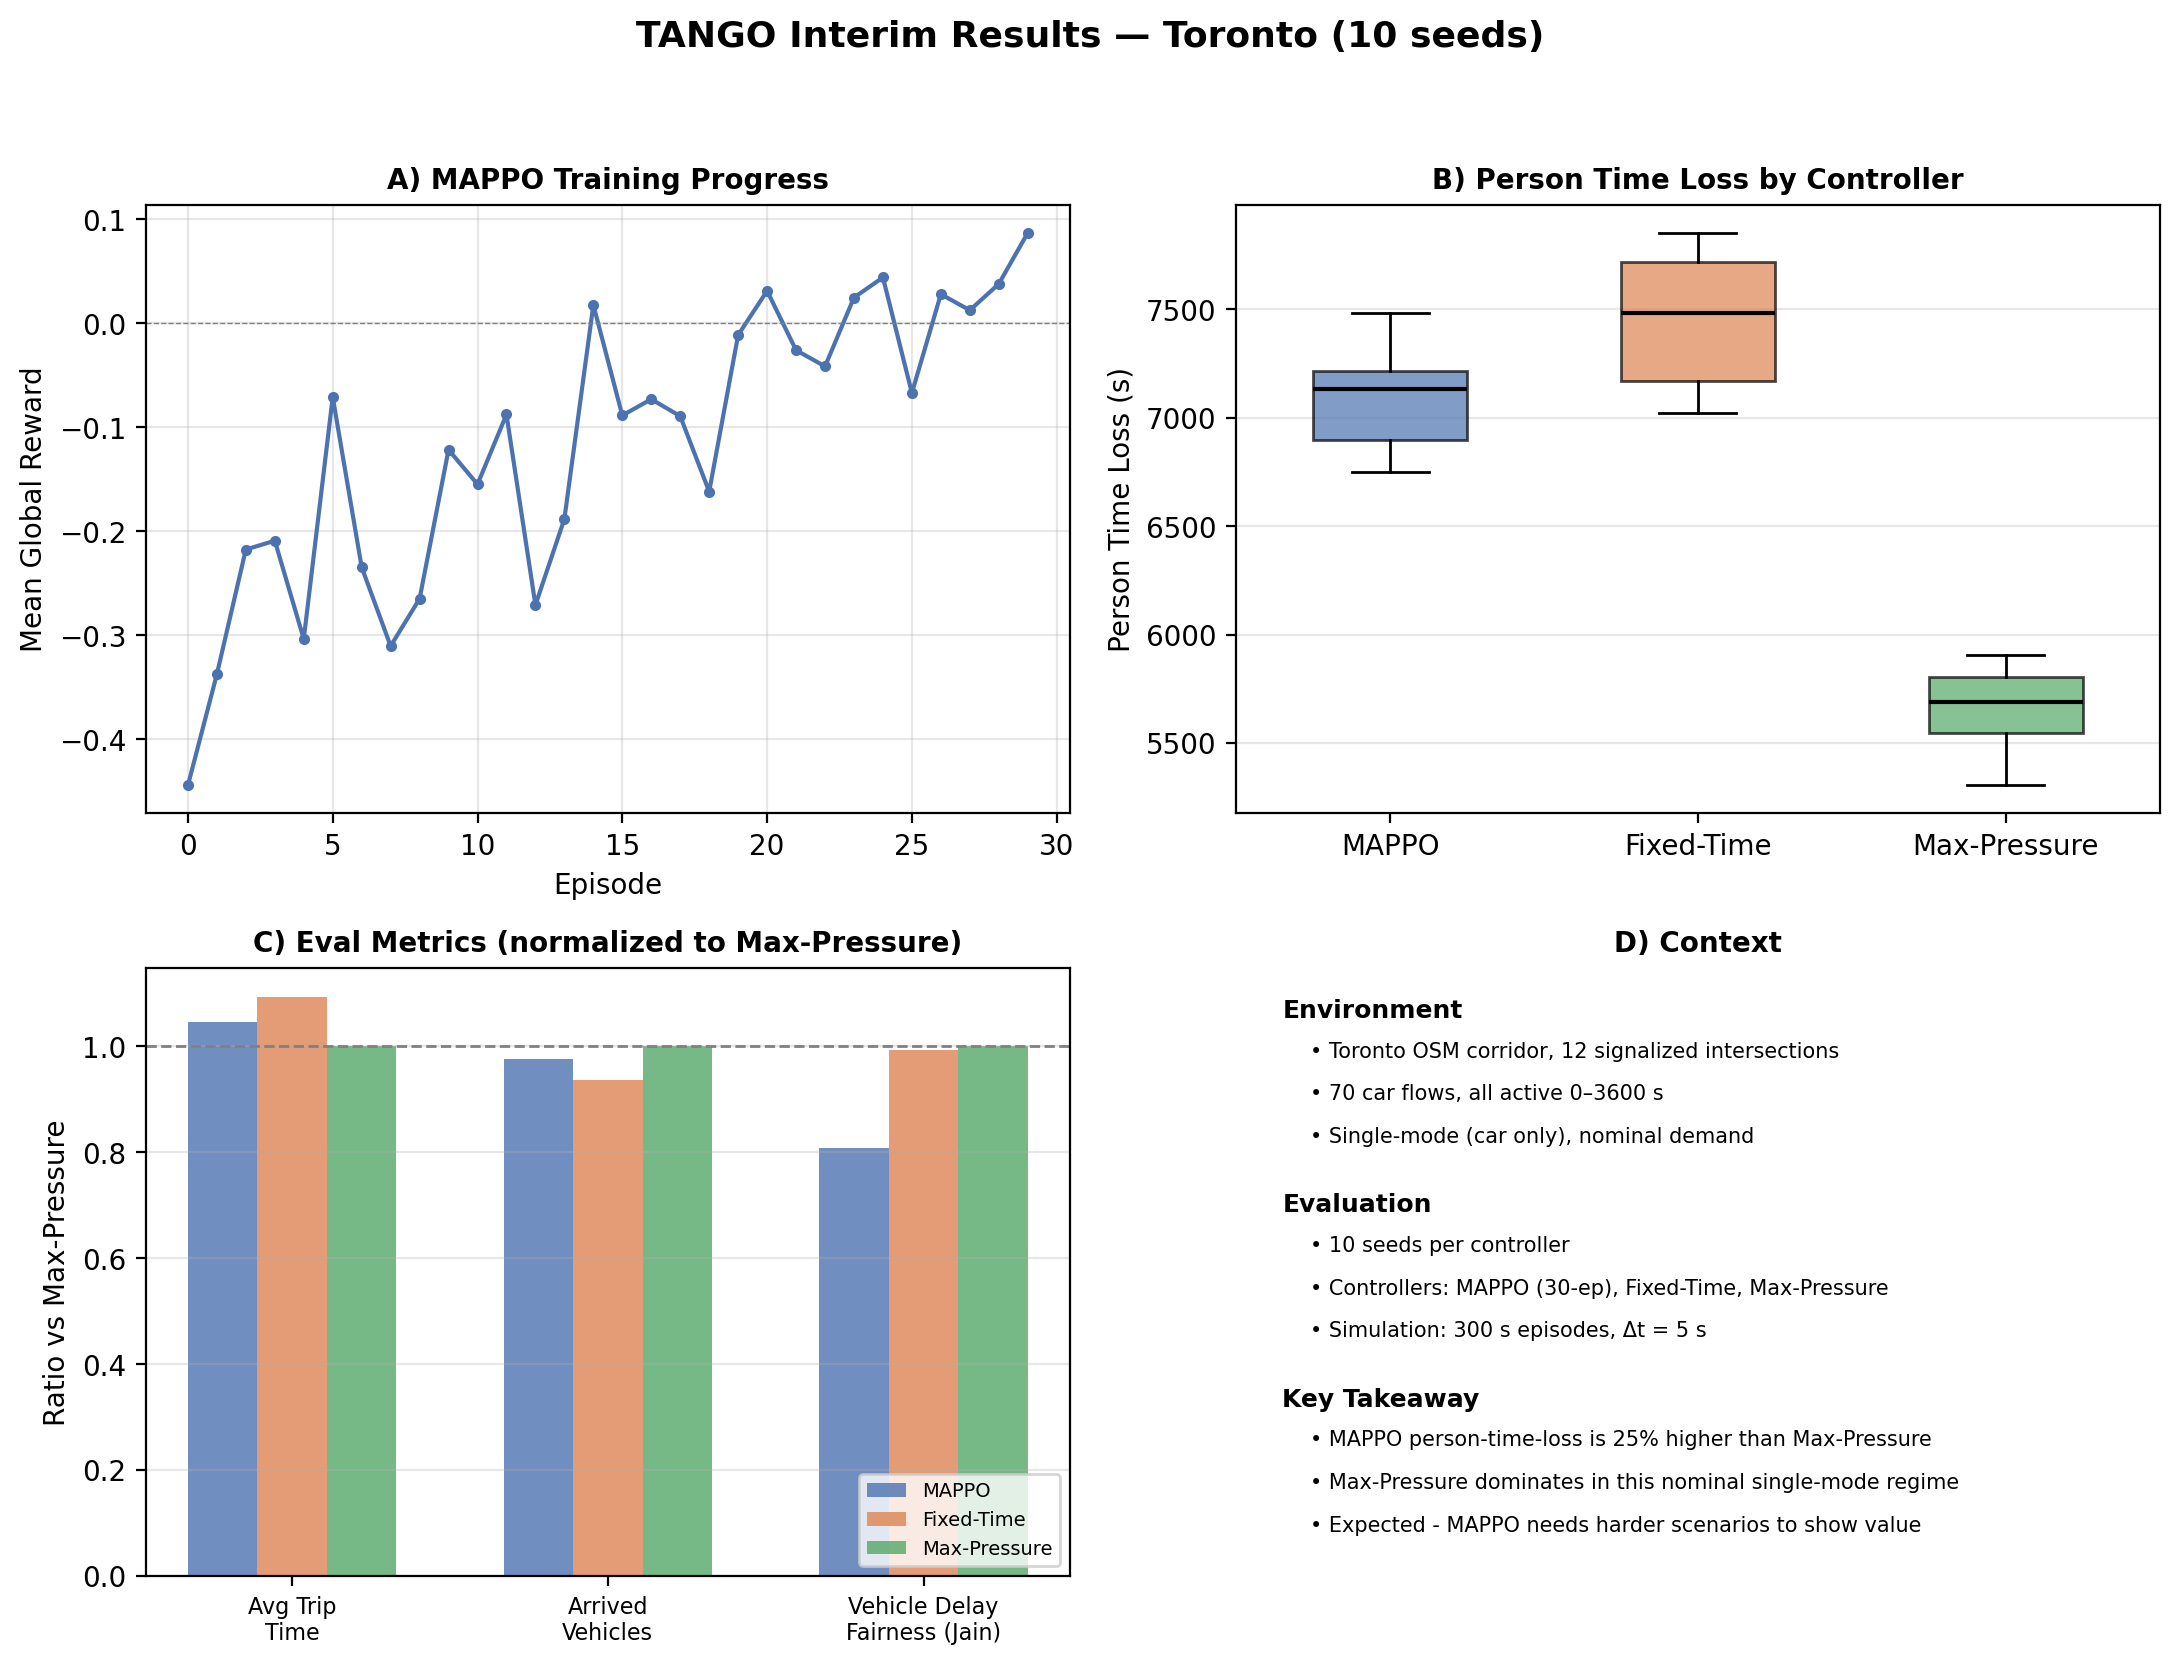
\includegraphics[width=\columnwidth]{reports/figures/interim_objective_results.png}
\caption{Interim results on the Toronto corridor (10 seeds per controller).
  \textbf{A)} MAPPO training progress (mean global reward).
  \textbf{B)} Person time loss distribution.
  \textbf{C)} Evaluation metrics normalized to Max-Pressure.
  \textbf{D)} Environment context.}
\label{fig:interim}
\end{figure}

Max-Pressure dominates all metrics under nominal conditions. This is expected:
it is provably throughput-optimal under stationary, single-commodity
demand~\cite{max_pressure_optimal}, which is exactly this benchmark. The
Toronto corridor with 70 uniform car flows is the regime where Max-Pressure's
local queue-balancing heuristic is near-optimal. No controller reaches the
proposal's Jain fairness target of 0.8, indicating that delay inequality
across vehicles is inherent to this network topology and demand pattern, not
controller-specific.

The 25\% gap motivates concrete next steps: (1)~warm-start MAPPO from
Max-Pressure imitation so it begins at least as good as the heuristic,
(2)~curriculum training with progressively harder scenarios (demand spikes,
incidents, multi-modal flows) where Max-Pressure's single-commodity assumption
breaks, and (3)~extend training beyond 30 episodes---the training curve
(Panel~A) shows the policy improving but not yet converged. The
multi-objective reward already demonstrates that richer signals substantially
improve learning; the next leverage point is the training environment, not the
reward.


% ============================================================================
% Appendices (do not count toward page limit)
% ============================================================================

% Place these after \section{References} / bibliography, before the NeurIPS checklist

\appendix

\section{Metric Definitions}
\label{app:metrics}

\begin{tabularx}{\columnwidth}{@{}l X@{}}
\toprule
\textbf{Metric} & \textbf{Definition} \\
\midrule
Person-time-loss (s) & Aggregated excess travel time over free-flow conditions (SUMO \texttt{timeLoss}), weighted by estimated person occupancy: 1.3 per car, 30 per transit vehicle. \\
Vehicle delay fairness (Jain) & Jain's index~\cite{jain1984} computed over per-vehicle final time-loss values for all vehicles that completed their trip during the episode. \\
Throughput & Number of vehicles that completed their trip within the episode. \\
Avg trip time (s) & Mean travel time (departure to arrival) across all arrived vehicles. \\
\bottomrule
\end{tabularx}

\section{MAPPO Hyperparameters}
\label{app:hyperparams}

\begin{tabular}{@{}ll@{}}
\toprule
\textbf{Parameter} & \textbf{Value} \\
\midrule
Hidden dimension          & 128 \\
Hidden layers             & 2 (actor and critic) \\
Activation                & ReLU \\
Actor learning rate       & $3 \times 10^{-4}$ \\
Critic learning rate      & $1 \times 10^{-3}$ \\
Optimizer                 & Adam \\
Discount ($\gamma$)       & 0.99 \\
GAE $\lambda$             & 0.95 \\
PPO clip $\epsilon$       & 0.2 \\
Entropy coefficient       & 0.01 \\
Value loss coefficient    & 0.5 \\
Gradient clip (max norm)  & 0.5 \\
PPO epochs per update     & 5 \\
Minibatch size            & 512 \\
Observation normalization & Welford running mean/variance \\
\bottomrule
\end{tabular}

\section{Reward Function}
\label{app:reward}

\textbf{Multi-objective reward} (used for main results):
\begin{equation}
r_i = -w_d \log(1 + d_i) + w_t \log(1 + \tau_i) + w_f \, J(\boldsymbol{\tau})
\label{eq:reward}
\end{equation}
where $d_i$ is the total waiting time on edges approaching intersection~$i$,
$\tau_i$ is the vehicle count on those edges,
$J(\boldsymbol{\tau})$ is Jain's index~\cite{jain1984} over per-agent
throughputs (shared across all agents as a coordination signal), and the
weights are $w_d = 1.0$, $w_t = 1.0$, $w_f = 0.25$.

\textbf{Time-loss reward} (initial approach, abandoned):
\begin{equation}
r_i = -w_d \log(1 + d_i)
\end{equation}
The log transform normalizes the delay scale for PPO stability while
preserving monotonicity with time loss.


% ============================================================================
% Bibliography entries needed (add to references.bib)
% ============================================================================
%
% @article{mappo,
%   title={The Surprising Effectiveness of PPO in Cooperative Multi-Agent Games},
%   author={Yu, Chao and Velu, Akash and Vinitsky, Eugene and others},
%   journal={Advances in Neural Information Processing Systems},
%   volume={35},
%   year={2022}
% }
%
% @article{ppo,
%   title={Proximal Policy Optimization Algorithms},
%   author={Schulman, John and Wolski, Filip and Dhariwal, Prafulla and others},
%   journal={arXiv preprint arXiv:1707.06347},
%   year={2017}
% }
%
% @article{jain1984,
%   title={A Quantitative Measure of Fairness and Discrimination for Resource Allocation in Shared Computer Systems},
%   author={Jain, Raj and Chiu, Dah-Ming and Hawe, William},
%   journal={DEC Research Report TR-301},
%   year={1984}
% }
%
% @article{max_pressure_optimal,
%   title={Max Pressure Control of a Network of Signalized Intersections},
%   author={Varaiya, Pravin},
%   journal={Transportation Research Part C},
%   volume={36},
%   pages={177--195},
%   year={2013}
% }
%
% @article{gae,
%   title={High-Dimensional Continuous Control Using Generalized Advantage Estimation},
%   author={Schulman, John and Moritz, Philipp and Levine, Sergey and others},
%   journal={arXiv preprint arXiv:1506.02438},
%   year={2016}
% }
%
% Already in proposal: citylight, sumo_home, libsignal/pytSC
